% GNUPLOT: LaTeX picture with Postscript
\documentclass{minimal}
% Set font size
\makeatletter
\def\@ptsize{1}
\InputIfFileExists{size11.clo}{}{%
   \GenericError{(gnuplot) \space\space\space\@spaces}{%
      Gnuplot Error: File `size11.clo' not found! Could not set font size%
   }{See the gnuplot documentation for explanation.%
   }{For using a font size a file `size<fontsize>.clo' has to exist.
        Falling back ^^Jto default fontsize 10pt.}%
  \def\@ptsize{0}
  \input{size10.clo}%
}%
\makeatother
% Load packages
\usepackage{calc}
\usepackage{graphicx}
\usepackage{color}
\usepackage{transparent}
\makeatletter
% Select an appropriate default driver (from TeXLive graphics.cfg)
\begingroup
  \chardef\x=0 %
  % check pdfTeX
  \@ifundefined{pdfoutput}{}{%
    \ifcase\pdfoutput
    \else
      \chardef\x=1 %
    \fi
  }%
  % check VTeX
  \@ifundefined{OpMode}{}{%
    \chardef\x=2 %
  }%
\expandafter\endgroup
\ifcase\x
  % default case
  \PassOptionsToPackage{dvips}{geometry}
\or
  % pdfTeX is running in pdf mode
  \PassOptionsToPackage{pdftex}{geometry}
\else
  % VTeX is running
  \PassOptionsToPackage{vtex}{geometry}
\fi
\makeatother
% Set papersize
\usepackage[papersize={311.00bp,425.00bp},text={311.00bp,425.00bp}]{geometry}
% No page numbers and no paragraph indentation
\pagestyle{empty}
\setlength{\parindent}{0bp}%
% Load configuration file
\InputIfFileExists{gnuplot.cfg}{%
  \typeout{Using configuration file gnuplot.cfg}%
}{%
 \typeout{No configuration file gnuplot.cfg found.}%
}%
\renewcommand\familydefault{\sfdefault}\usepackage{cmbright}
\begin{document}
\begingroup
  \makeatletter
  \providecommand\color[2][]{%
    \GenericError{(gnuplot) \space\space\space\@spaces}{%
      Package color not loaded in conjunction with
      terminal option `colourtext'%
    }{See the gnuplot documentation for explanation.%
    }{Either use 'blacktext' in gnuplot or load the package
      color.sty in LaTeX.}%
    \renewcommand\color[2][]{}%
  }%
  \providecommand\includegraphics[2][]{%
    \GenericError{(gnuplot) \space\space\space\@spaces}{%
      Package graphicx or graphics not loaded%
    }{See the gnuplot documentation for explanation.%
    }{The gnuplot epslatex terminal needs graphicx.sty or graphics.sty.}%
    \renewcommand\includegraphics[2][]{}%
  }%
  \providecommand\rotatebox[2]{#2}%
  \@ifundefined{ifGPcolor}{%
    \newif\ifGPcolor
    \GPcolortrue
  }{}%
  \@ifundefined{ifGPblacktext}{%
    \newif\ifGPblacktext
    \GPblacktextfalse
  }{}%
  % define a \g@addto@macro without @ in the name:
  \let\gplgaddtomacro\g@addto@macro
  % define empty templates for all commands taking text:
  \gdef\gplbacktext{}%
  \gdef\gplfronttext{}%
  \makeatother
  \ifGPblacktext
    % no textcolor at all
    \def\colorrgb#1{}%
    \def\colorgray#1{}%
  \else
    % gray or color?
    \ifGPcolor
      \def\colorrgb#1{\color[rgb]{#1}}%
      \def\colorgray#1{\color[gray]{#1}}%
      \expandafter\def\csname LTw\endcsname{\color{white}}%
      \expandafter\def\csname LTb\endcsname{\color{black}}%
      \expandafter\def\csname LTa\endcsname{\color{black}}%
      \expandafter\def\csname LT0\endcsname{\color[rgb]{1,0,0}}%
      \expandafter\def\csname LT1\endcsname{\color[rgb]{0,1,0}}%
      \expandafter\def\csname LT2\endcsname{\color[rgb]{0,0,1}}%
      \expandafter\def\csname LT3\endcsname{\color[rgb]{1,0,1}}%
      \expandafter\def\csname LT4\endcsname{\color[rgb]{0,1,1}}%
      \expandafter\def\csname LT5\endcsname{\color[rgb]{1,1,0}}%
      \expandafter\def\csname LT6\endcsname{\color[rgb]{0,0,0}}%
      \expandafter\def\csname LT7\endcsname{\color[rgb]{1,0.3,0}}%
      \expandafter\def\csname LT8\endcsname{\color[rgb]{0.5,0.5,0.5}}%
    \else
      % gray
      \def\colorrgb#1{\color{black}}%
      \def\colorgray#1{\color[gray]{#1}}%
      \expandafter\def\csname LTw\endcsname{\color{white}}%
      \expandafter\def\csname LTb\endcsname{\color{black}}%
      \expandafter\def\csname LTa\endcsname{\color{black}}%
      \expandafter\def\csname LT0\endcsname{\color{black}}%
      \expandafter\def\csname LT1\endcsname{\color{black}}%
      \expandafter\def\csname LT2\endcsname{\color{black}}%
      \expandafter\def\csname LT3\endcsname{\color{black}}%
      \expandafter\def\csname LT4\endcsname{\color{black}}%
      \expandafter\def\csname LT5\endcsname{\color{black}}%
      \expandafter\def\csname LT6\endcsname{\color{black}}%
      \expandafter\def\csname LT7\endcsname{\color{black}}%
      \expandafter\def\csname LT8\endcsname{\color{black}}%
    \fi
  \fi
    \setlength{\unitlength}{0.0500bp}%
    \ifx\gptboxheight\undefined%
      \newlength{\gptboxheight}%
      \newlength{\gptboxwidth}%
      \newsavebox{\gptboxtext}%
    \fi%
    \setlength{\fboxrule}{0.5pt}%
    \setlength{\fboxsep}{1pt}%
\begin{picture}(6220.00,8500.00)%
    \gplgaddtomacro\gplbacktext{%
      \csname LTb\endcsname%%
      \put(736,6658){\makebox(0,0)[r]{\strut{}$10$}}%
      \csname LTb\endcsname%%
      \put(736,7404){\makebox(0,0)[r]{\strut{}$100$}}%
      \csname LTb\endcsname%%
      \put(736,8150){\makebox(0,0)[r]{\strut{}$1000$}}%
      \csname LTb\endcsname%%
      \put(838,6438){\makebox(0,0){\strut{}}}%
      \csname LTb\endcsname%%
      \put(1877,6438){\makebox(0,0){\strut{}}}%
      \csname LTb\endcsname%%
      \put(2917,6438){\makebox(0,0){\strut{}}}%
      \csname LTb\endcsname%%
      \put(3956,6438){\makebox(0,0){\strut{}}}%
      \csname LTb\endcsname%%
      \put(4996,6438){\makebox(0,0){\strut{}}}%
      \csname LTb\endcsname%%
      \put(6035,6438){\makebox(0,0){\strut{}}}%
      \csname LTb\endcsname%%
      \put(62,8329){\makebox(0,0)[l]{\strut{}(a)}}%
      \csname LTb\endcsname%%
      \put(62,6544){\makebox(0,0)[l]{\strut{}(b)}}%
      \csname LTb\endcsname%%
      \put(62,4632){\makebox(0,0)[l]{\strut{}(c)}}%
      \csname LTb\endcsname%%
      \put(62,2720){\makebox(0,0)[l]{\strut{}(d)}}%
    }%
    \gplgaddtomacro\gplfronttext{%
      \csname LTb\endcsname%%
      \put(264,7515){\rotatebox{-270}{\makebox(0,0){\strut{}MFPT $\mu / \tau$}}}%
      \csname LTb\endcsname%%
      \put(2273,8206){\makebox(0,0)[r]{\strut{}$A \rightarrow B$}}%
      \csname LTb\endcsname%%
      \put(3367,8206){\makebox(0,0)[r]{\strut{}$B \rightarrow A$}}%
      \csname LTb\endcsname%%
      \put(4461,8206){\makebox(0,0)[r]{\strut{}$C \rightarrow D$}}%
      \csname LTb\endcsname%%
      \put(5555,8206){\makebox(0,0)[r]{\strut{}$D \rightarrow C$}}%
    }%
    \gplgaddtomacro\gplbacktext{%
      \csname LTb\endcsname%%
      \put(736,4748){\makebox(0,0)[r]{\strut{}$10$}}%
      \csname LTb\endcsname%%
      \put(736,5525){\makebox(0,0)[r]{\strut{}$100$}}%
      \csname LTb\endcsname%%
      \put(736,6302){\makebox(0,0)[r]{\strut{}$1000$}}%
      \csname LTb\endcsname%%
      \put(838,4526){\makebox(0,0){\strut{}}}%
      \csname LTb\endcsname%%
      \put(1877,4526){\makebox(0,0){\strut{}}}%
      \csname LTb\endcsname%%
      \put(2917,4526){\makebox(0,0){\strut{}}}%
      \csname LTb\endcsname%%
      \put(3956,4526){\makebox(0,0){\strut{}}}%
      \csname LTb\endcsname%%
      \put(4996,4526){\makebox(0,0){\strut{}}}%
      \csname LTb\endcsname%%
      \put(6035,4526){\makebox(0,0){\strut{}}}%
      \csname LTb\endcsname%%
      \put(62,8329){\makebox(0,0)[l]{\strut{}(a)}}%
      \csname LTb\endcsname%%
      \put(62,6544){\makebox(0,0)[l]{\strut{}(b)}}%
      \csname LTb\endcsname%%
      \put(62,4632){\makebox(0,0)[l]{\strut{}(c)}}%
      \csname LTb\endcsname%%
      \put(62,2720){\makebox(0,0)[l]{\strut{}(d)}}%
    }%
    \gplgaddtomacro\gplfronttext{%
      \csname LTb\endcsname%%
      \put(264,5640){\rotatebox{-270}{\makebox(0,0){\strut{}STD $\sigma /\tau$}}}%
    }%
    \gplgaddtomacro\gplbacktext{%
      \csname LTb\endcsname%%
      \put(736,3263){\makebox(0,0)[r]{\strut{}$2$}}%
      \csname LTb\endcsname%%
      \put(736,3727){\makebox(0,0)[r]{\strut{}$3$}}%
      \csname LTb\endcsname%%
      \put(736,4191){\makebox(0,0)[r]{\strut{}$4$}}%
      \csname LTb\endcsname%%
      \put(838,2613){\makebox(0,0){\strut{}}}%
      \csname LTb\endcsname%%
      \put(1877,2613){\makebox(0,0){\strut{}}}%
      \csname LTb\endcsname%%
      \put(2917,2613){\makebox(0,0){\strut{}}}%
      \csname LTb\endcsname%%
      \put(3956,2613){\makebox(0,0){\strut{}}}%
      \csname LTb\endcsname%%
      \put(4996,2613){\makebox(0,0){\strut{}}}%
      \csname LTb\endcsname%%
      \put(6035,2613){\makebox(0,0){\strut{}}}%
      \csname LTb\endcsname%%
      \put(62,8329){\makebox(0,0)[l]{\strut{}(a)}}%
      \csname LTb\endcsname%%
      \put(62,6544){\makebox(0,0)[l]{\strut{}(b)}}%
      \csname LTb\endcsname%%
      \put(62,4632){\makebox(0,0)[l]{\strut{}(c)}}%
      \csname LTb\endcsname%%
      \put(62,2720){\makebox(0,0)[l]{\strut{}(d)}}%
    }%
    \gplgaddtomacro\gplfronttext{%
      \csname LTb\endcsname%%
      \put(418,3727){\rotatebox{-270}{\makebox(0,0){\strut{}skewness $\kappa$}}}%
    }%
    \gplgaddtomacro\gplbacktext{%
      \csname LTb\endcsname%%
      \put(736,1186){\makebox(0,0)[r]{\strut{}$0.05$}}%
      \csname LTb\endcsname%%
      \put(736,1486){\makebox(0,0)[r]{\strut{}$0.1$}}%
      \csname LTb\endcsname%%
      \put(736,1785){\makebox(0,0)[r]{\strut{}$0.15$}}%
      \csname LTb\endcsname%%
      \put(736,2084){\makebox(0,0)[r]{\strut{}$0.2$}}%
      \csname LTb\endcsname%%
      \put(736,2384){\makebox(0,0)[r]{\strut{}$0.25$}}%
      \csname LTb\endcsname%%
      \put(838,701){\makebox(0,0){\strut{}$0$}}%
      \csname LTb\endcsname%%
      \put(1877,701){\makebox(0,0){\strut{}$50$}}%
      \csname LTb\endcsname%%
      \put(2917,701){\makebox(0,0){\strut{}$100$}}%
      \csname LTb\endcsname%%
      \put(3956,701){\makebox(0,0){\strut{}$150$}}%
      \csname LTb\endcsname%%
      \put(4996,701){\makebox(0,0){\strut{}$200$}}%
      \csname LTb\endcsname%%
      \put(6035,701){\makebox(0,0){\strut{}$250$}}%
      \csname LTb\endcsname%%
      \put(62,8329){\makebox(0,0)[l]{\strut{}(a)}}%
      \csname LTb\endcsname%%
      \put(62,6544){\makebox(0,0)[l]{\strut{}(b)}}%
      \csname LTb\endcsname%%
      \put(62,4632){\makebox(0,0)[l]{\strut{}(c)}}%
      \csname LTb\endcsname%%
      \put(62,2720){\makebox(0,0)[l]{\strut{}(d)}}%
    }%
    \gplgaddtomacro\gplfronttext{%
      \csname LTb\endcsname%%
      \put(142,1815){\rotatebox{-270}{\makebox(0,0){\strut{}occupation $\Pi$}}}%
      \csname LTb\endcsname%%
      \put(3488,422){\makebox(0,0){\strut{}$f~/ ( \epsilon / \mathcal{L} )$}}%
      \csname LTb\endcsname%%
      \put(2967,2464){\makebox(0,0)[r]{\strut{}$A$}}%
      \csname LTb\endcsname%%
      \put(3653,2464){\makebox(0,0)[r]{\strut{}$B$}}%
      \csname LTb\endcsname%%
      \put(4339,2464){\makebox(0,0)[r]{\strut{}$C$}}%
      \csname LTb\endcsname%%
      \put(5025,2464){\makebox(0,0)[r]{\strut{}$D$}}%
    }%
    \gplbacktext
    \put(0,0){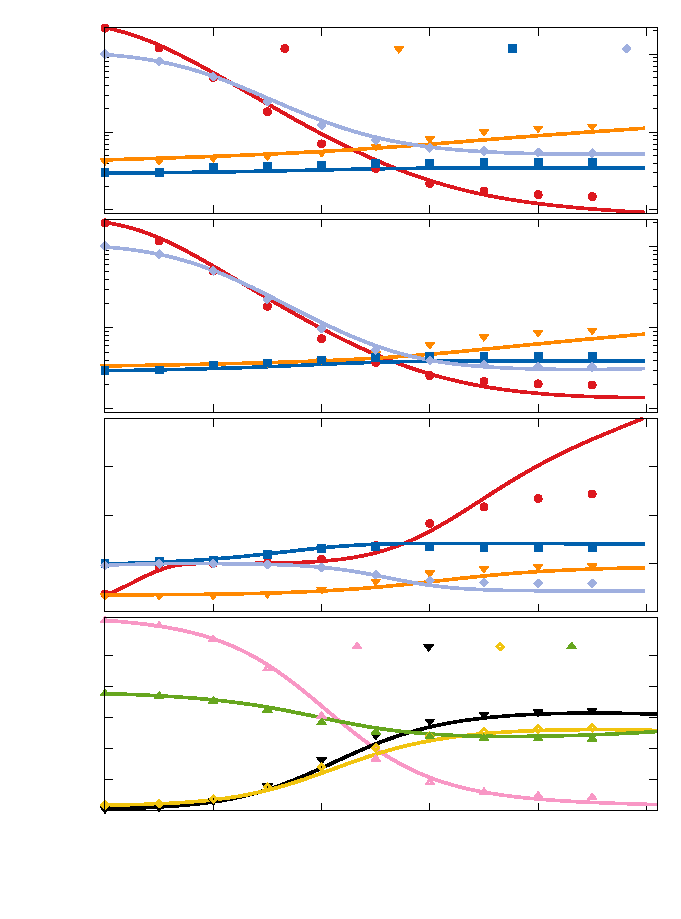
\includegraphics{mom_9040-inc}}%
    \gplfronttext
  \end{picture}%
\endgroup
\end{document}
